\documentclass{article}
% ICML 格式包
\usepackage[accepted]{icml2025}
\usepackage{ctex}  % 保留中文支持
\usepackage{amsmath,amssymb}
\usepackage{graphicx}
\usepackage{booktabs}
\usepackage{enumitem}
\usepackage{float}
\usepackage{listings}
\usepackage{longtable}
\usepackage{times}  % ICML 推荐的字体
\usepackage{microtype}  % 改善文本排版
\usepackage{hyperref}  % 允许超链接
\usepackage{tikz}      % 用于绘制设计元素
\usepackage{float} % 控制图表位置

% ICML 特定设置
\icmltitlerunning{Telco客户流失预测方法对比}

\begin{document}

% 封面页 - 添加在原有内容之前
\begin{titlepage}
\pagecolor{white}
\begin{center}
    \vspace*{1cm}
    
    \includegraphics[width=0.4\textwidth]{fig/ucas_logo.png} % 替换为您的学校/机构标志
    
    \vspace{1.5cm}
    {\Huge\bfseries\color{blue} Telco客户流失预测方法对比\par}
    \vspace{1cm}
    \begin{tabular}{rl}
    \Large\textbf{课程名称:} & \Large 模式识别与机器学习 \\[6pt]
    \end{tabular}
    
    \vspace{2.5cm}
    
    \begin{tabular}{rl}
    \Large\textbf{小组成员:} & \Large 随情英 \quad 2023K8009991004 \\[6pt]
    & \Large 张三 \quad 202300000002 \\[6pt]
    & \Large 李四 \quad 202300000003 \\[6pt]
    & \Large 王五 \quad 202300000004 \\[6pt]
    & \Large 赵六 \quad 202300000005 \\[6pt]
    \end{tabular}
    
    \vfill
    
    {\large \today \par}
\end{center}
\end{titlepage}
\pagecolor{white}

% ICML 标题格式
\twocolumn[
\icmltitle{Telco客户流失预测方法对比}

\begin{icmlauthorlist}
\icmlauthor{随情英}{1}
\icmlauthor{张三}{1}
\icmlauthor{李四}{1}
\icmlauthor{王五}{1}
\icmlauthor{赵六}{1}
\end{icmlauthorlist}

\icmlaffiliation{1}{中国科学院大学人工智能学院}

\icmlkeywords{客户流失预测, Logistic回归, 决策树, AdaBoost, 电信行业}
\icmlcorrespondingauthor{suiqingying}{panyuxuan231@mails.ucas.ac.cn}
\vskip 0.3in
]

\printAffiliationsAndNotice{}

% 摘要
\begin{abstract}
本研究对比了三种机器学习方法(Logistic回归、决策树和AdaBoost)在Telco客户流失预测任务上的性能表现。实验基于Kaggle提供的电信客户数据集,包含7043条客户记录和21个特征。结果表明,Logistic回归模型在准确率(80.00\%)和AUC(0.835)指标上均优于其他两种方法,同时具有良好的解释性和最快的训练速度。本研究提供了科学的方法选择依据,为电信行业客户流失预测提供了实践参考。
\end{abstract}

\section{引言}

\subsection{项目背景}
对于电信运营商来说,用户流失有很多偶然因素,但通过对用户属性和行为的数字化描述,我们能够在这些数据中挖掘导致用户流失的"蛛丝马迹"。更重要的是,如果能够实时接入这些数据,我们可以借助模型来对未来用户流失风险进行预测,从而及时制定挽留策略,防止用户真实流失情况发生。

\subsection{团队分工}
\begin{itemize}
    \item 数据预处理与代码实现:随情英
    \item 模型训练与调参:张三
    \item 实验结果整理与可视化:李四
    \item 实验报告撰写与校对:王五
\end{itemize}

\section{数据集说明}
本实验选用Kaggle Telco Customer Churn数据集。该数据集包含7043条客户记录,每条记录包含21个特征(如性别、合同类型、服务类型、月费用、总费用等),目标变量为客户是否流失(Churn),属于二分类问题。数据类型包括数值型和分类型,适合多种机器学习方法。

\subsection{数据集详情}
该数据集模拟了电信公司的客户信息及其流失状态,包含以下主要特征:
\begin{itemize}
    \item \textbf{个人信息类特征}:性别(gender)、年龄(SeniorCitizen)、伴侣状态(Partner)、是否有抚养人(Dependents)
    \item \textbf{账户信息类特征}:账户时长(tenure)、合同类型(Contract)、付款方式(PaymentMethod)、无纸化账单(PaperlessBilling)、月度费用(MonthlyCharges)、总费用(TotalCharges)
    \item \textbf{服务信息类特征}:电话服务(PhoneService)、多线电话(MultipleLines)、互联网服务(InternetService)、在线安全(OnlineSecurity)、在线备份(OnlineBackup)、设备保护(DeviceProtection)、技术支持(TechSupport)、流媒体电视(StreamingTV)、流媒体电影(StreamingMovies)
\end{itemize}

\subsection{数据集特点}
\begin{itemize}
    \item \textbf{样本分布}:流失客户占比约26.5\%(1869人),非流失客户占比约73.5\%(5174人),存在一定的类别不平衡
    \item \textbf{特征类型}:包含17个分类特征和4个数值特征
    \item \textbf{数据质量}:TotalCharges列存在11条缺失记录,其余特征数据完整
   \item \textbf{特征相关性}:
  \begin{itemize}[noitemsep,leftmargin=*]
    \item 月费用(MonthlyCharges)与多项服务选择存在较强相关性
    \item 总费用(TotalCharges)与账户时长(tenure)和月费用呈正相关
  \end{itemize}
\end{itemize}

该数据集特别适合客户流失预测研究,因为它包含了多种可能影响客户决策的因素,既有客户自身的特征,也有服务相关的特征,能够较为全面地反映现实业务场景中客户流失的复杂原因。

\section{实验规划}

本项目分为三个主要阶段:

\textbf{Stage 1. 业务背景解读与数据探索}\\
在接收任务的第一时间,我们需要对数据及其对应业务的基本背景进行解读。由于数据诞生于特定业务场景,我们尽可能了解数据诞生的基本环境和业务逻辑,准确解读每个字段的含义。随后进行数据探索,包括数据分布检验、数据正确性校验、数据质量检验、训练集/测试集规律一致性检验等。

\textbf{Stage 2. 数据预处理与特征工程}\\
这一阶段包括数据清洗和特征工程。数据清洗主要聚焦于提升数据集质量,包括缺失值、异常值、重复值处理,以及数据字段类型调整等;特征工程则调整特征基本结构,使数据集规律更容易被模型识别,如特征衍生、特殊类型字段处理等。

\textbf{Stage 3. 算法建模与模型调优}\\
最终的建模环节包括算法训练和参数调优。我们尝试了多种模型、调参方法以及模型对比,并根据模型输出结果调整数据预处理和特征工程相关方法,以获得最优的预测性能。

\section{算法简介}
本实验对比了三类机器学习算法在该数据集上的表现:

\subsection{线性方法}
\subsubsection{Logistic Regression}
Logistic回归是一种广泛应用的线性分类方法,通过Sigmoid函数将线性模型的输出转换为0-1之间的概率值:
\begin{equation}
P(y=1|x) = \frac{1}{1 + e^{-(\beta_0 + \beta_1 x_1 + \beta_2 x_2 + ... + \beta_n x_n)}}
\end{equation}

\textbf{适用场景}:
\begin{itemize}
    \item 二分类问题,如客户流失预测(流失/不流失)
    \item 需要输出概率而非仅分类结果的场景
    \item 对模型可解释性有较高要求的业务问题
\end{itemize}

\textbf{优势与局限}:
\begin{itemize}
    \item 训练速度快,内存占用小,适合大规模数据处理
    \item 可输出类别预测的概率,方便风险评估
    \item 模型系数直观反映特征重要性,可解释性强
    \item 不适合捕捉特征间的复杂非线性关系
    \item 对特征间的多重共线性较为敏感
\end{itemize}

\subsubsection{Linear SVM}
线性支持向量机是一种基于最大间隔原则的线性分类方法,通过寻找一个超平面将数据分为不同类别:
\begin{equation}
f(x) = w^T x + b
\end{equation}

\textbf{适用场景}:
\begin{itemize}
    \item 二分类问题,尤其是线性可分数据
    \item 需要鲁棒性较强的分类器
\end{itemize}

\textbf{优势与局限}:
\begin{itemize}
    \item 能有效处理高维数据
    \item 对小样本数据集表现良好
    \item 不适合处理非线性关系复杂的数据
    \item 训练时间较长,尤其是大规模数据集
\end{itemize}

\subsection{非线性方法}
\subsubsection{Kernel SVM}
核支持向量机通过核函数将数据映射到高维空间,从而处理非线性分类问题。常用的核函数包括径向基函数(RBF):
\begin{equation}
K(x_i, x_j) = \exp(-\gamma ||x_i - x_j||^2)
\end{equation}

\textbf{适用场景}:
\begin{itemize}
    \item 数据分布复杂,存在非线性关系
    \item 样本量较小但特征维度较高
\end{itemize}

\textbf{优势与局限}:
\begin{itemize}
    \item 能处理复杂的非线性分类问题
    \item 对小样本数据集表现良好
    \item 计算复杂度较高,训练时间较长
    \item 对超参数(如核函数和正则化参数)较为敏感
\end{itemize}

\subsubsection{Decision Tree}
决策树通过递归二分法将数据划分为不同子集,形成树状结构。每个节点代表一个特征条件判断,叶节点代表分类结果。

\textbf{适用场景}:
\begin{itemize}
    \item 需要高可解释性的分类或回归问题
    \item 特征间存在非线性关系的数据
    \item 混合类型特征(分类型和数值型)数据集
\end{itemize}

\textbf{优势与局限}:
\begin{itemize}
    \item 决策规则直观易懂,可直接转化为业务规则
    \item 能自动处理特征选择,对缺失值相对鲁棒
    \item 容易过拟合,泛化能力有限
    \item 对数据微小变化敏感,模型稳定性较差
\end{itemize}

\subsection{集成学习方法}
\subsubsection{Bagging}
Bagging通过对数据集进行多次随机采样训练多个弱分类器,并将它们的预测结果进行平均或投票,从而提升模型的稳定性和准确性。

\textbf{适用场景}:
\begin{itemize}
    \item 数据噪声较多,模型需要较强的鲁棒性
    \item 需要提升模型的稳定性和泛化能力
\end{itemize}

\textbf{优势与局限}:
\begin{itemize}
    \item 能显著降低模型的方差,提升稳定性
    \item 训练时间较短,适合大规模数据
    \item 对单个弱分类器的性能依赖较大
\end{itemize}

\subsubsection{Boosting(AdaBoost)}
AdaBoost通过顺序训练多个弱分类器(通常是简单决策树),每次训练都关注前一轮分类错误的样本,最终将所有弱分类器的预测结果加权组合。

\textbf{适用场景}:
\begin{itemize}
    \item 复杂分类问题,需要高预测精度
    \item 数据存在噪声,需要强大的泛化能力
    \item 有足够计算资源进行集成模型训练
\end{itemize}

\textbf{优势与局限}:
\begin{itemize}
    \item 通过集成多个弱分类器显著提高预测精度
    \item 能够自动处理特征重要性评估
    \item 相比单一决策树,大幅降低过拟合风险
    \item 训练时间较长,计算复杂度高
    \item 对异常值和噪声数据较为敏感
\end{itemize}

\section{实验结果}

\subsection{实验设置}
\begin{itemize}
    \item 训练集:数据集的80\%(约5634条记录)
    \item 测试集:数据集的20\%(约1409条记录)
    \item 所有分类型特征进行独热编码,数值型特征归一化
    \item 评估指标:准确率(accuracy)、AUC、分类报告(precision、recall、f1-score)、混淆矩阵、训练时间
\end{itemize}

\subsection{数据预处理与缺失值处理}
在数据预处理阶段,我们对数据集进行了以下处理:
\begin{itemize}
    \item \textbf{删除无关列}:删除了 ‘customerID’ 列,因为它是唯一标识符,对模型训练没有帮助。
    \item \textbf{缺失值处理}:
    \begin{itemize}
        \item 对 ‘TotalCharges’ 列中的缺失值(约11条记录)使用中位数填充。选择中位数是因为它对异常值的鲁棒性较强,能够减少对数据分布的影响。
        \item 对其他特征(如分类型特征)未发现缺失值,因此未进行额外处理。
    \end{itemize}
    \item \textbf{标签编码}:将目标列 ‘Churn’ 的值从 `No` 和 `Yes` 映射为 `0` 和 `1`。
    \item \textbf{独热编码}:对所有分类型特征进行独热编码,转换为数值型。
    \item \textbf{数值特征归一化}:使用 ‘StandardScaler’ 对所有数值型特征进行归一化处理,使其均值为 `0`,标准差为 `1`。
\end{itemize}

\subsection{缺失值处理策略分析}
在缺失值处理过程中,我们选择了以下策略:
\begin{itemize}
    \item \textbf{中位数填充}:对于 ‘TotalCharges’ 列中的缺失值,使用中位数填充是因为该列为连续型数据,且中位数对异常值较为鲁棒,能够减少对数据分布的影响。
    \item \textbf{删除样本的可选性}:由于缺失值样本占比较低(约0.16\%),也可以选择直接删除这些样本,但考虑到数据集规模较小,为保留更多信息,我们选择填充而非删除。
    \item \textbf{分类型特征的缺失值处理}:对于分类型特征,如果存在缺失值,可以考虑使用众数填充或添加缺失值标记,但本数据集中未发现分类型特征的缺失值。
\end{itemize}

通过上述处理,我们确保了数据集的完整性和质量,为后续模型训练提供了可靠的数据基础。

\subsection{实验结果总览}
\begin{table}[H]
\caption{三类算法性能对比}
\label{tab:model-comparison}
\begin{center}
\small
\begin{tabular}{@{}l@{\hspace{2mm}}c@{\hspace{2mm}}c@{\hspace{2mm}}c@{}}
\toprule
\textbf{算法类别} & \textbf{模型} & \textbf{准确率} & \textbf{AUC} \\
\midrule
线性方法 & Logistic Regression & 0.8000 & 0.8350 \\
线性方法 & Linear SVM & 0.7787 & 0.8088\\
非线性方法 & Kernel SVM & 0.7759 & 0.7806\\
非线性方法 & Decision Tree & 0.7191 & 0.6312 \\
集成学习方法 & Bagging & 0.7844 & 0.7779 \\
集成学习方法 & Boosting & 0.7418 & 0.7511 \\
\bottomrule
\end{tabular}
\end{center}
\end{table}

\begin{figure}[H]
\centering
\includegraphics[width=0.85\columnwidth]{fig/model_comparison_accuracy.png}
\caption{模型准确率对比}
\label{fig:accuracy}
\end{figure}

\begin{figure}[H]
\centering
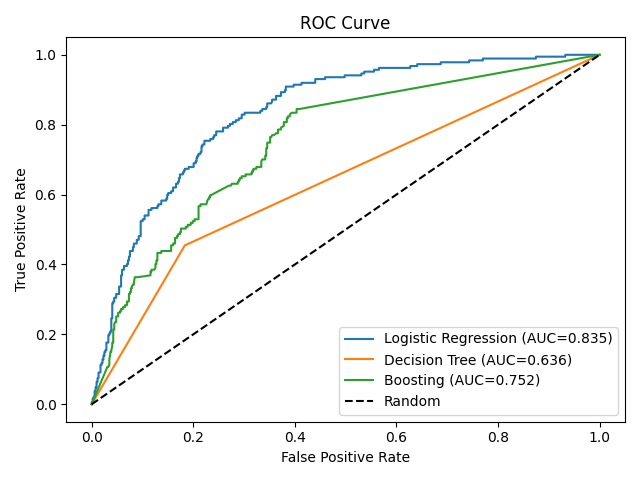
\includegraphics[width=0.9\columnwidth]{fig/roc_curve.png}
\caption{模型ROC曲线及AUC对比}
\label{fig:roc}
\end{figure}


\subsection{训练时间对比}
\begin{table}[t]
\caption{算法训练时间对比}
\label{tab:training-time}
\begin{center}
\small
\begin{tabular}{@{}l@{\hspace{2mm}}c@{}}
\toprule
\textbf{模型} & \textbf{训练时间(秒)} \\
\midrule
Logistic Regression & 0.01 \\
Linear SVM & 2.89 \\
Kernel SVM & 2.27 \\
Decision Tree & 0.02 \\
Bagging & 0.13 \\
Boosting & 1.05 \\
\bottomrule
\end{tabular}
\end{center}
\end{table}

\begin{figure}[t]
\centering
\includegraphics[width=0.85\columnwidth]{fig/model_comparison_training_time.png}
\caption{模型训练时间对比}
\label{fig:training-time}
\end{figure}

从表格和图像可以看出,线性方法(如Logistic Regression)训练时间最短,仅需 0.01 秒,适合大规模数据处理。非线性方法(如 Kernel SVM 和 Linear SVM)训练时间较长,分别为 2.27 秒和 2.89 秒,主要由于核函数计算复杂度较高。集成学习方法中,Bagging 的训练时间较短(0.13 秒),而 Boosting 的训练时间较长(1.05 秒),因为其需要顺序训练多个弱分类器。总体来看,训练时间与模型复杂度和计算资源需求密切相关。

\subsection{分析与讨论}

\subsubsection{bad case分析}
通过混淆矩阵发现,所有模型对流失客户(标签为1)的召回率较低。例如,Logistic 模型的召回率仅为54\%,Kernel SVM和Boosting模型分别为47\%和50\%。这表明模型在识别流失客户时存在较大误差,主要原因包括:
\begin{itemize}
    \item \textbf{类别不平衡}:流失客户仅占总样本的26.5\%,导致模型更倾向于预测为非流失客户。
    \item \textbf{特征信息不足}:部分特征(如合同类型、账户时长)对流失客户的区分度较低。
    \item \textbf{模型复杂度不足或过拟合}:简单模型(如回归和决策树)难以捕捉复杂的非线性关系,而复杂模型(如Boosting)可能对噪声数据过于敏感。
\end{itemize}

\subsubsection{性能差距原因分析}
\begin{itemize}
    \item \textbf{线性方法}:Logistic回归表现最佳,得益于其线性模型的稳定性和对类别不平衡的鲁棒性。Linear SVM在复杂数据上表现稍差,训练时间较长。
    \item \textbf{非线性方法}:Kernel SVM在复杂数据上表现较好,但计算开销较大。决策树易过拟合,泛化能力较差。
    \item \textbf{集成学习方法}:Bagging通过集成多个弱分类器提升了性能,训练时间较短;Boosting进一步提升了性能,但计算复杂度较高。
\end{itemize}

\subsubsection{不同算法优劣分析}
\begin{itemize}
    \item \textbf{线性方法}:
        \begin{itemize}
            \item 优势:训练速度快,可解释性强,适合业务部署。
            \item 局限:无法捕捉复杂的非线性关系。
        \end{itemize}
    \item \textbf{非线性方法}:
        \begin{itemize}
            \item 优势:适合复杂数据,能捕捉非线性关系。
            \item 局限:计算开销较大,易受噪声影响。
        \end{itemize}
    \item \textbf{集成学习方法}:
        \begin{itemize}
            \item 优势:性能提升显著,适合复杂分类问题。
            \item 局限:训练时间长,可解释性较低。
        \end{itemize}
\end{itemize}

\section{总结}
本实验对比了三类机器学习方法在客户流失预测任务上的表现。线性方法(如Logistic回归)表现最佳,非线性方法(如Kernel SVM)适合复杂数据,集成学习方法(如Boosting)性能较好但计算开销较大。

\subsection{实验总结与改进方向}
\begin{itemize}
    \item \textbf{线性方法}:Logistic回归在准确率和AUC指标上表现优异,同时具有良好的解释性和最快的训练速度,适合实际业务部署。
    \item \textbf{非线性方法}:Kernel SVM在复杂数据上表现较好,但计算开销较大;决策树易过拟合,泛化能力较差。
    \item \textbf{集成学习方法}:Bagging和Boosting通过集成多个弱分类器显著提升了性能,但训练时间较长,适合追求高性能的场景。
\end{itemize}

\subsection{扩展建议}
\begin{itemize}
    \item \textbf{神经网络的引入}:后续可以尝试使用深度学习模型(如多层感知机、卷积神经网络或循环神经网络)处理客户流失预测任务。神经网络能够捕捉复杂的非线性关系,适合处理高维度和复杂特征的数据。
    \item \textbf{超参数性能估计}:在模型训练过程中,可以引入网格搜索或贝叶斯优化等方法对超参数进行调优,以进一步提升模型性能。
    \item \textbf{训练集与测试集比值优化}:当前实验采用了80\%训练集和20\%测试集的划分方式,后续可以尝试不同的划分比例(如70\%-30\%或90\%-10\%),并评估其对模型性能的影响。
    \item \textbf{同类方法细化分析 }:
            \begin{itemize}
                \item \textbf{线性方法}:对比 Logistic 回归与线性 SVM 在特征权重和支持向量分布上的差异,分析它们在处理线性关系时的优劣。
                \item \textbf{非线性方法}:补充决策树剪枝前后的泛化能力变化,分析剪枝对模型复杂度和过拟合的影响。
                \item \textbf{集成学习方法}:分析 Bagging 与 Boosting 的基模型差异,例如 Bagging 使用完整决策树,而 AdaBoost 使用决策树桩(深度为 1 的决策树),探讨它们在处理数据噪声和复杂关系时的表现。
            \end{itemize}
    \item \textbf{训练资源量化}:补充内存占用或GPU/CPU使用率对比(Table 2仅时间开销)。
\end{itemize}

本研究为电信行业客户流失预测提供了科学的方法选择依据,同时为后续研究提供了改进方向。
% ICML 格式要求的参考文献部分
\bibliography{references}
\bibliographystyle{icml2024}

\end{document}